\chapter{Background}

\section{Linux testing}

The Linux ecosystem has been around for a long time and as a consequence, every new version inherits a vast codebase. Being an open source system it heavily relies on the community to validate the functionality and improve it along the way. The bugs are mainly reported by the users, but by the time the new software reaches end user the bug might be much more difficult to fix. To ease the work of developers automated testing suites emerged that validated subsystems and provided continuous integration.

Ideally, a developer would test the new code as early as possible - before submitting the patch. However, such early testing is usually not extensive or rigorous enough and might not happen at all. Untested patches often lead to notable developer effort wasted on bugs that are found later in the cycle when it is significantly less efficient to fix them.

Several large projects developed over time to automate the Linux Kernel testing such as LTP - Linux Testing Project and Autotest. However, testing for compliance is currently done inside companies that provide distributions for the IT industry, such examples are Wind River and MontaVista. This embedded software vendors use in-house, closed source validators, yet the profiler characteristics are made public so that clients benefit from the transparency of the testing process. For instance, Wind River provides a carrier grade profile for their Linux distributions so clients can see how the system they intend to purchase was validated. This information can be used for creating a open-source tool with the same purpose that can have a larger impact.

\section{Linux distributions and specifications}

Each specification aims to provide a guideline for future developers and tries to shape and direct a specific technological branch so that future development is not hindered in any way, is secure and based on sound principles. A specification usually consists of a set of rules, guidelines and principles. They can ease the development and maintenance effort of the whole community by bringing uniformity and structure to the systems it is used for. It is intended to be as extensive as possible but there is a natural limitation to how much a specification can cover. Usually they focus on a very specific system that is part of a larger branch. This focus makes the specification easier to implement and ensures a more detailed coverage and higher quality. The present paper discusses only the software specifications created for production-ready Linux distributions.

\subsection{The Yocto Project}
The Yocto Project is an open source collaboration project that aims to facilitate creation of embedded Linux distributions. The project relies heavily on previous work done in different open source communities. It brings together tools and a template system to allow the creation of custom Linux based operating systems. Because Yocto has a very broad approach and the purpose of creating a whole distribution is difficult to achieve, a reference Yocto distribution was created called \textbf{Poky}. In itself, Yocto only states that a custom image must be created based on a template and aims to facilitate interoperability between the tools under the project umbrella, Poky offers a concrete implementation of this idea. It offers a simple yet comprehensive example of how Yocto is supposed to work and can be used for fast prototyping. The main components of Poky are \textbf{BitBake}, \textbf{OpenEmbedded Core} and Yocto specific metadata. The proposed framework is integrated with Poky and uses its subsystems to provide the testing functionality.

\subsubsection*{Bitbake}
Bitbake is a cross-compilation tool able to parse Python and Shell scripts. It is inspired by the package management system used in Gentoo Linux distribution - Portage. Bitbake uses a system of recipes to keep track of the required packages and the dependencies between them. The recipes provide the template system of Yocto, they are the main input data based on witch a custom distribution is created. Since Bitbake is able to fetch source code from most common repository types such as github and mercurial and install most common package formats such as .deb and .rpm, the available code base is extensive. It also means that as long as builds happen often, the software will be up to date.

Arguably Bitbake's greatest advantage is the dependency management of the tasks. After parsing the recipes (which can be a combination of Python and Shell script) Bitbake is able to create concurrent tasks that process operations such as code fetching, building and installing and order them based on their dependencies. Considering how large a single build of Poky can become (over 24GB) the efficiency of Bitbake makes the system viable.

\subsubsection*{OpenEmbedded Core}
OpenEmbedded (OE) is an open source project that pre-dates Yocto and is based on Bitbake recipes. After the creation of the Yocto Project, the community behind OpenEmbedded had the opportunity to change the architecture. In the beginning all the recipes of the system were all gathered in the same place, but the system became unmaintainable. The recipes were therefore split intro layers and the codebase of OE was split between OE-core and meta-oe. The core provides all the basic functionality required by anyone who tries to build an embedded distribution, while meta-oe contains all the rest of the recipes. OpenEmbedded project offers an extensive list of available layers.

By default, Poky contains the OE core, but it also preserves the layered architecture through which almost any common functionality, software and tools can be added. The proposed framework uses one such layer called meta-ellida to integrate with Yocto.

\subsection{CGL - Carrier Grade Linux}
The first of the two specifications discussed and supported by the framework is CGL - Carrier Grade Linux.
Given its broad approach, Carrier Grade Linux can be thought of as a convergence of other specifications. The original intent was to identify functionality already available in the open source community that is of particular interest to carriers. Most of the requirements laid out in the CGL specification apply equally well to systems ranging from large corporate infrastructures to small, highly mobile devices.

The CGL specification is very much requirement oriented. The structure follows a few abstract characteristics that a system should have and then specifies in great detail how these attributes can be achieved or at least tested. The main requirements of a carrier grade distribution are listed next.

\begin{enumerate}
\item \textbf{Standard}

The first section of the document addresses compliance with many other specifications or standards such as the Linux Standard Base (LSB), specific pieces of POSIX standards, IPv6 and IP Security standards (IPsec), Requests for Comment (RFCs), and PCI Express specifications.
\item \textbf{Hardware}

The hardware requirements describe hardware-specific support considered necessary for carrier environments.
\item \textbf{Serviceability}

The serviceability section develops on topics regarding the accessibility, remote maintenance and monitoring of possibly difficult to access systems. 
\item \textbf{Performance}

Performance wise, a number of attributes of the operating system that must be configurable at run-time are specified, along with process scheduling, signal processing order, priorities and methods for timely processing.
\item \textbf{Security}

The security segment aims to make systems more resistant to a wide range of attacks and increase the reliability. They cover aspects ranging from technical details such as avoiding buffer overflows to architectural and system wide facilities such as using access control and role-based access control or using technologies such as Trusted Platform Module.
\item \textbf{Availability}

The availability focuses on methods and features that lower the probability of having sudden or unexpected loss of functionality. Having a very high uptime is one of the vital aspects of a carrier system.
\item \textbf{Cluster}

The Cluster requirement category has a similar purpose to the Availability section, but instead of focusing on individual systems it refers to cluster based systems. It states the requirements for providing high availability using a multi-system cluster.

\end{enumerate}

Considering the scale and volatility of today's communications CGL proved to be of invaluable help. This is why the Linux Foundation has started setting the groundwork for standards and specifications that will hopefully guide other industrial branches. New IT industries are emerging around concepts such as smart cities and connected automotive products and they come with a highly disruptive potential. CGL's development paved the way for a multitude of standards and specifications that may help bring unity to a very dynamic, yet important factor of our life.

\subsection{AGL - Automotive Grade Linux}
The second specification discussed is relatively new and not yet as polished and mature as CGL, it aims to bring consistency to the automotive Linux ecosystem - AGL - Automotive Grade Linux. AGL is a Linux Foundation Collaborative Project that tries to provide the main automobile producers with a set of rules to follow when creating embedded distributions that run inside cars, but is also dedicated to creating open source software solutions for automotive applications. The initiative led to the creation of a reference Linux distribution based on Yocto. It enables rapid prototyping and is an opportunity for the industry players to collaborate towards a safer, more user-oriented software system. The AGL Workgroup has the support or several large vendors from the automotive and semiconductor industries.

The architecture of the specification is based on four layers. Each layer covers a separate part of the distribution and has rules concerning practical aspects of the system.

\begin{figure}[h!]
  \centering
	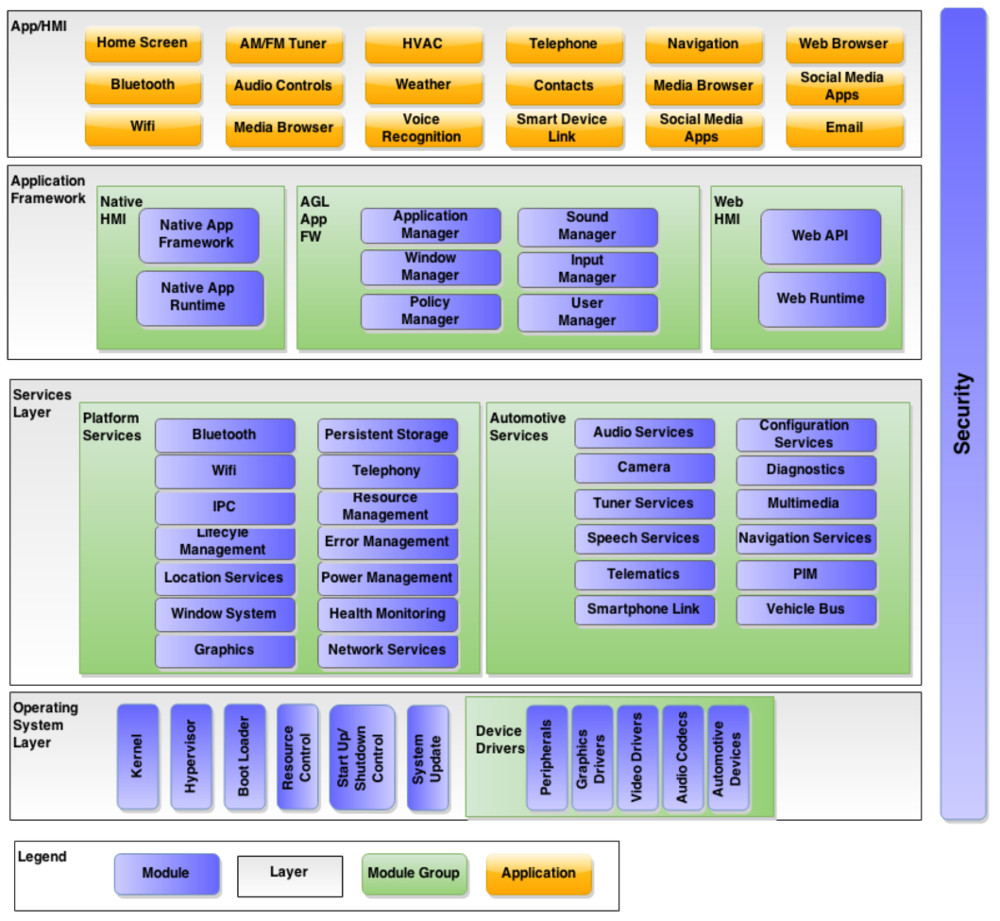
\includegraphics[width=0.9\textwidth]{images/agl_arch.jpg}
    \caption{AGL Architecture}
\end{figure}

\begin{enumerate}
\item \textbf{App/HMI}

The layer contains applications along with the business logic behind them and the human-machine interface (HMI). It is mainly comprised of guidelines regarding the user interface and the frameworks that link together the UI and the applications. 
\item \textbf{Application Framework}

The AGL Application Framework is meant to provide basic functionality to all applications regardless of the framework they were built with. It is intended to standardize \textbf{how} system-wide services are provided.
\item \textbf{Services}

The Services Layer contains user space services that all applications can access. It defines \textbf{which} services are available system-wide and their behaviour. Generally the services provide either an IPC type interface or a subroutine/function API.
\item \textbf{Security}

AGL only provides a very brief guide to security, stating only that a system-wide access control system should be in place.
\item \textbf{Operating system}

The OS layer deals with the more low level requirements of the system, regulating the behaviour of the memory, storage, file systems, kernel etc.
\end{enumerate}

AGL currently only targets In-Vehicle-Infotainment (IVI) systems, but additional use cases such as instrument clusters and telematics will eventually be supported. Linux Foundation expressed great interest in supporting and developing AGL over time. Therefore, it is not far-fetched to expect that it will have an impact in the embedded market and that testing tools will be in demand.

\subsubsection*{Pre-AGL initiatives - GENIVI}
Before 2012, when AGL collaborative open source project started bringing together automakers, another initiative with roughly the same purpose called GENIVI was created (2009). GENIVI is a non-profit industry alliance committed to driving the broad adoption of open source, In-Vehicle Infotainment (IVI) software and providing open technology for the connected car. GENIVI project currently maintains a fairly extensive list of open source applications created specifically for cars and benefits from both the support of a large community and sponsoring from large car manufacturers. GENIVI filled a gap in the automotive industry by pioneering the use of free and open source software for non-safety-critical automotive systems. It is currently more popular among European car makers, while AGL is being adopted by most Asian producers. However, considering the two to be competitors on the automotive market would not be very accurate. GENIVI applications can be used alongside or inside the AGL systems. They complete each other and strengthen the presence of open source software in a market where vendor specific products used to be ubiquitous. The effort to make reliable, secure and easy to use software while being cost effective and with a short time-to-market cycle has proven to be a hard limitation in all industries where software development is necessary. Therefore, AGL and GENIVI will have a wider impact by functioning alongside one another. The trend these initiatives started will not fade too soon and is creating a technological void.

\subsection{AGL - CGL comparison}
Even if the resulting set of guidelines are similar, the two specifications have different approaches. AGL has the software system as starting point and describes how it should behave in a broad sense. This is made obvious by the layered structure, with each layer being a part of the software system. CGL on the other hand has the requirements as starting point. It starts by defining what is important for the user or what is expected in abstract terms such as being reliable and secure. The specification then develops on each requirement through a set of rules and offers very detailed test scenarios along with the expected results. For the moment, AGL is still at version 1.0 and lacks a very formal structure, mainly because it is not intended to be used for a compliance program, but as a general guideline for the AGL project. CGL currently stands at the fifth version and has been in constant refining for almost 20 years. Since then, it has become a de facto standard for telecommunications providers. The comparison is relevant because it outlines how specifications might differ and how the framework's representation of them should be able to handle these differences.

\section{Related work}

\subsection{Fuego and AGL-JTA}
Fuego is the official automated test framework for the LTSI project. LTSI stands for Long Term Support Initiative and its purpose is to maintain a common Linux base for use in a variety of consumer electronics products. Fuego is a test framework specifically designed for embedded Linux testing, it uses a Jenkins front-end and a server-client model for running tests on multiple different boards at once. It also comes pre-packed with around 60 tests.

The main goals of Fuego are to facilitate community based testing by providing a simple system to run tests remotely and easily share both tests and results. These are achieved through hardware abstraction, the use of an extensible and user friendly front-end and the ability to use it as a hosted service. Even if Fuego has been around for a short time, and is still a work in progress, a branch called AGL-JTA was created for testing the official AGL distribution. The project is for the moment about a year old, has close to no documentation and exists in the form of a Fuego installation with certain plugin customisations and a small suite of tests.

Fuego and AGL-JTA are very close in purpose to the framework discussed. In truth, they can be used to offer the same functionality since they are meant to provide remote automatic software testing. However, Fuego is less focused on the high level functionality of full spec validation and more hardware oriented. Fuego is not dependent on Yocto generated systems although it supports Yocto, but instead has an architectural model that encapsulates hardware abstraction so that the LTSI kernels can be run on various boards. It also contains a custom built compile and schedule engine for running tests. These extensions, while providing relevant functionality, are cumbersome to use, increase the complexity a lot and are not mandatory for the task of validating distributions. The proposed frameworks aims to be hardware agnostic, it could as well use only VMs as long as they run the targeted distribution.

\begin{figure}[h!]
  \centering
	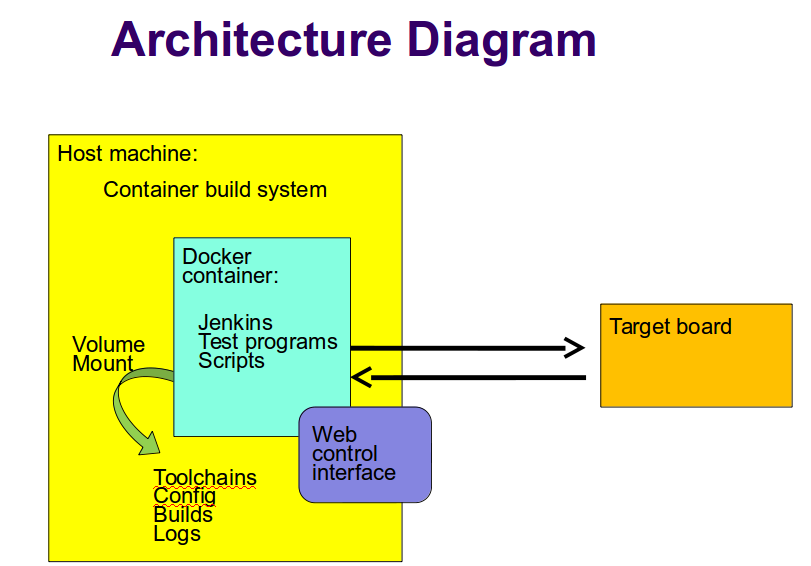
\includegraphics[width=0.7\textwidth]{images/fuego-arch.png}
    \caption{Fuego Architecture}
\end{figure}

\subsection{LAVA}

LAVA stands for Linaro Automation and Validation Architecture and is a continuous integration framework created by Linaro. It is intended to test OS - hardware configurations by installing operating systems on a variety of hardware, but can also install individual tests for in depth testing. LAVA can build and test kernels on supported hardware with a pre-set frequency and is designed for validation during development, thus the label of continuous integration. LAVA has features such as parallel scheduling, hardware sharing, live result reporting among others. The proposed framework tries to match the versatility and scalability of LAVA. 
\subsection{LTP}

The Linux Test Project is an open source project that has the support of companies such as IBM, Cisco, Fujitsu, SUSE, Red Hat. It aims to deliver test suites that validate Linux systems in terms of reliability, robustness, and stability. The LTP test suite contains a collection of tools - manly individual tests - that can be used for testing the Linux kernel and related features. The test collection consists of C programs and bash scripts that can be used either through CLI or through control files that define what tests should run. The C tests are automatically compiled and provide a very wide range of tests - over 4000 programs and scripts. Any testing framework should be able to harness this resource.

